% CVPR 2022 Paper Template
% based on the CVPR template provided by Ming-Ming Cheng (https://github.com/MCG-NKU/CVPR_Template)
% modified and extended by Stefan Roth (stefan.roth@NOSPAMtu-darmstadt.de)

\documentclass[10pt,twocolumn,letterpaper,final]{article} % final 추가% \documentclass[10pt,twocolumn,letterpaper, final]{article}

%%%%%%%%% PAPER TYPE  - PLEASE UPDATE FOR FINAL VERSIONf
\usepackage[review]{cvpr}      % To produce the REVIEW version
%\usepackage{cvpr}              % To produce the CAMERA-READY version
%\usepackage[pagenumbers]{cvpr} % To force page numbers, e.g. for an arXiv version

% Include other packages here, before hyperref.
\usepackage{graphicx}
\usepackage{amsmath}
\usepackage{amssymb}
\usepackage{booktabs}
\usepackage{caption}
\usepackage{float} % Required for [H] option in figure placement
\usepackage{multicol} % For managing column layout
\usepackage{parskip} % 문단 간의 간격 추가
\usepackage{setspace} % 공백 조정

% 공백 조절: 그림과 텍스트 사이 간격 줄이기
\setlength{\floatsep}{1pt} % 두 개의 float 사이 간격
\setlength{\textfloatsep}{1pt} % 텍스트와 float 사이 간격
\setlength{\intextsep}{2pt} % 텍스트 내 float 간격

\captionsetup{width=\linewidth} % 캡션 폭을 텍스트 폭에 맞추기


% It is strongly recommended to use hyperref, especially for the review version.
% hyperref with option pagebackref eases the reviewers' job.
% Please disable hyperref *only* if you encounter grave issues, e.g. with the
% file validation for the camera-ready version.
%
% If you comment hyperref and then uncomment it, you should delete
% ReviewTempalte.aux before re-running LaTeX.
% (Or just hit 'q' on the first LaTeX run, let it finish, and you
%  should be clear).
\usepackage[pagebackref,breaklinks,colorlinks]{hyperref}


% Support for easy cross-referencing
\usepackage[capitalize]{cleveref}
\crefname{section}{Sec.}{Secs.}
\Crefname{section}{Section}{Sections}
\Crefname{table}{Table}{Tables}
\crefname{table}{Tab.}{Tabs.}


%%%%%%%%% PAPER ID  - PLEASE UPDATE
\def\cvprPaperID{12345} % *** Enter the CVPR Paper ID here
\def\confName{CVPR}
\def\confYear{2022}


\begin{document}

%%%%%%%%% TITLE - PLEASE UPDATE
\title{\ Do Pre-trained ImageNet Weights Enhance Road Semantic Segmentation?}

\author{JunSeok Kim\\
Electrical and Electronic Engineering
Yonsei University\\
Seoul, Republic of Korea
\\
{\tt\small kkjs3700@naver.com}
% For a paper whose authors are all at the same institution,
% omit the following lines up until the closing ``}''.
% Additional authors and addresses can be added with ``\and'',
% just like the second author.
% To save space, use either the email address or home page, not both
\and
Second Author\\
Institution2\\
First line of institution2 address\\
{\tt\small secondauthor@i2.org}
}
\maketitle

%%%%%%%%% ABSTRACT
\begin{abstract}
   In autonomous driving systems, road semantic segmentation plays an important role in accurately identifying road and environmental structures. This study analyzes the impact of pre-trained ImageNet weights on segmentation performance by utilizing U-Net and U-Net++ models. Three models (U-Net, U-Net++ without pre-trained weights, and U-Net++ with pre-trained weights) were compared using the KITTI dataset, and training was performed for 200 epochs. Model performance was analyzed using the Intersection-over-Union (IoU) metric and qualitative evaluation. Experimental results show that the U-Net++ model with pre-trained weights achieves the highest IoU and best captures road boundaries and object details. This study shows that transfer learning of pre-trained Imagenet dataset weights can significantly improve the performance of models that capture road structure.
\end{abstract}

%%%%%%%%% BODY TEXT
\section{Introduction}
\label{sec:intro}
Semantic segmentation plays a key role in road recognition and boundary detection for autonomous vehicles. The above task of categorizing meaning on a pixel-by-pixel basis within an image is essential for applications such as autonomous vehicles. 
U-Net and U-Net++ are popular models in semantic segmentation, showing excellent performance in learning information about object boundaries, textures, and patterns in images.
U-Net utilizes an encoder-decoder structure and skip connections to preserve high-resolution details in images. At the same time, it is designed to learn high-level contextual information. U-Net++ extends this by adding nested skip connections and dense paths, which reduce the information gap between the encoder and decoder and provide more detailed segmentation results.

Initial weight settings have a significant impact on model performance, and transfer learning is an effective way to utilize these settings. This method is effective in leveraging pre-trained weights to accelerate learning on new datasets and improve generalization performance. In the ImageNet dataset, the pre-trained weights cover a wide range of visual features. This is useful in a variety of computer vision tasks, such as semantic segmentation.

Transfer learning is a powerful tool, but it doesn't always guarantee better performance. It can actually degrade performance if there is a large difference in features between the target task and the pre-trained dataset. 

In this study, we compare the road segmentation performance of U-Net, U-Net++ without pre-trained weights using VGG16 as a backbone, and U-Net++ with ImageNet pre-trained weights as initial values.  The results demonstrate that pre-trained ImageNet weights are beneficial for roadway semantic segmentation. 
This suggests the possibility of further research utilizing different backbone models and datasets in the future.

%-------------------------------------------------------------------------
%%%%%%%%% BODY TEXT
\section{Background}
\label{sec:intro}

In this background part, we will describe the models, the dataset, and the backbone model.
%-------------------------------------------------------------------------
\subsection{Structure and differences between UNet and UNet++ models}
The structure of UNet consists of a downsampling path that shrinks the input image to extract features, and an upsampling path that expands it back to restore them. Skip connections pass the output feature map from the downsampling path to the corresponding upsampling path. This design preserves high-resolution detail and makes the segmentation results precise.
UNet++ extends this structure, introducing Nested Skip Connections and Nested Decoders. Each decoder block in UNet++ learns richer information by simultaneously referencing the output of multiple depths of encoders, as well as the output of the previous decoder stage. This greatly improves segmentation performance by combining different spatial resolutions.

The main difference between the two models is in their 'Dense Skip Connections' and 'Nested Architecture'. These structures are designed to reduce the semantic gap between the encoder and decoder, and to learn more fine-grained feature information. This allows UNet++ to combine feature maps of different depths, which can lead to more sophisticated segmentation results.

%-------------------------------------------------------------------------
\subsection{Datasets Utilized}

\textbf{KITTI Dataset.} The KITTI dataset is developed for autonomous driving research. It contains real-world road data collected by a vehicle's front-facing camera and LiDAR sensor. The dataset is suitable for addressing various challenges such as Object Detection, Semantic Segmentation, and Depth Estimation. In particular, the segmentation data in the KITTI dataset provides high-quality training data by labeling major road objects such as roads, vehicles, and pedestrians on a pixel-by-pixel basis. In this study, we utilize the segmentation labels in the KITTI dataset to train a model that more clearly distinguishes the boundaries of roads and objects. These data, when combined with the complex architecture of UNet, enable a more precise understanding of the road environment.

\textbf{ImageNet Dataset.} ImageNet is a large visual dataset consisting of approximately 14 million natural images and more than 1,000 classes: animals (dogs, cats, elephants), plants (trees, flowers), objects (chairs, cars), places (beaches, mountains), etc.) The dataset is designed to allow models to learn from low-level features (lines, textures, etc.) to high-level features (object shapes, etc.). Models pre-trained with ImageNet are used in a transfer learning method in a variety of computer vision tasks. By using ImageNet weights as initialization, the model starts with common visual features already learned, allowing it to learn quickly in new domains. In this study, we use VGG16 weights trained with ImageNet as initialization for the UNet++ backbone to achieve both learning efficiency and segmentation performance.

%-------------------------------------------------------------------------
\subsection{VGG16 and pre-trained weights}

VGG16 is a model developed by Simonyan and Zisserman that performed well in the 2014 ImageNet Challenge. The model consists of 16 layers (13 convolutional layers and 3 fully connected layers) and is characterized by a deep structure designed using small 3x3 filters. 
VGG16 is pre-trained with the ImageNet dataset, which provides an effective learning state that recognizes common visual features such as edges, textures, patterns, etc. 
By using VGG16 as a backbone in a segmentation model, you can take advantage of the abundant visual features from the early stages of training. This can reduce training time and contribute to good performance.


%-------------------------------------------------------------------------
%%%%%%%%% BODY TEXT
\section{Method}
\label{sec:intro}

In this study, we compare the performance of three segmentation models using the augmented KITTI dataset.
\begin{enumerate}
    \item \textbf{UNet}: Basic model trained from the beginning, without using pre-trained weights.
    
    \item \textbf{UNet++ (no pre-trained weights)}: An extension of UNet, trained from the beginning with a model with a nested structure.
    
    \item \textbf{UNet++ (with pre-trained weights)}: Trained using ImageNet pre-trained weights from VGG16 as initial values
\end{enumerate} The main purpose of this experiment is to evaluate how changes in model structure and the use of pre-trained weights affect segmentation performance. 
The reason for evaluating the UNet model together is that we needed a comparison group to determine if taking the Netsted structure always results in good performance. Each model was trained for 200 epochs. Performance metrics were evaluated periodically during the training process to determine whether the learning converged.
%-------------------------------------------------------------------------
\subsection{Training and evaluation}

We used the augmented KITTI dataset for training. Augmentation techniques such as 'flipping, random cropping, and resizing' were applied to increase data diversity.
During the training process, we analyzed the trend of validation loss to verify the learning stability. Specifically, we used 'IoU metrics' and 'visual evaluation' to confirm that each model was stable during learning. After training, we loaded the best performing checkpoints from each model and performed segmentation predictions on the test images. The predicted results were finally compared through 'quantitative metrics' and 'qualitative evaluation'.


%-------------------------------------------------------------------------
\subsection{Evaluation metrics}
To evaluate the model performance, we used two evaluation methods.

\begin{enumerate}
    \item \textbf{Quantitative evaluation.} 
    The Intersection-over-Union (IoU) measures the overlap between the predicted segmentation mask and the ground truth. The formula is defined as
    \[
    \text{\textbf{IoU}} = \frac{\text{\textbf{Area of overlapping regions}}}{\text{\textbf{Area of union regions}}}
    \]
    Higher IoU values indicate more accurate segmentation.

    \item \textbf{Qualitative evaluation.} 
    We visually compared the predicted masks with the Ground Truth. The Ground Truth was represented by a red mask, which allowed us to evaluate in detail how well the predictions fit.
\end{enumerate}
%-------------------------------------------------------------------------
%%%%%%%%% BODY TEXT
\section{Result}
\label{sec:intro}
In this study, we evaluated three models: UNet, UNet++ (without pre-trained weights), and UNet++ (with pre-trained weights). We found that the UNet++ model with pre-trained weights performed the best.

\begin{figure}[H]
    \centering
    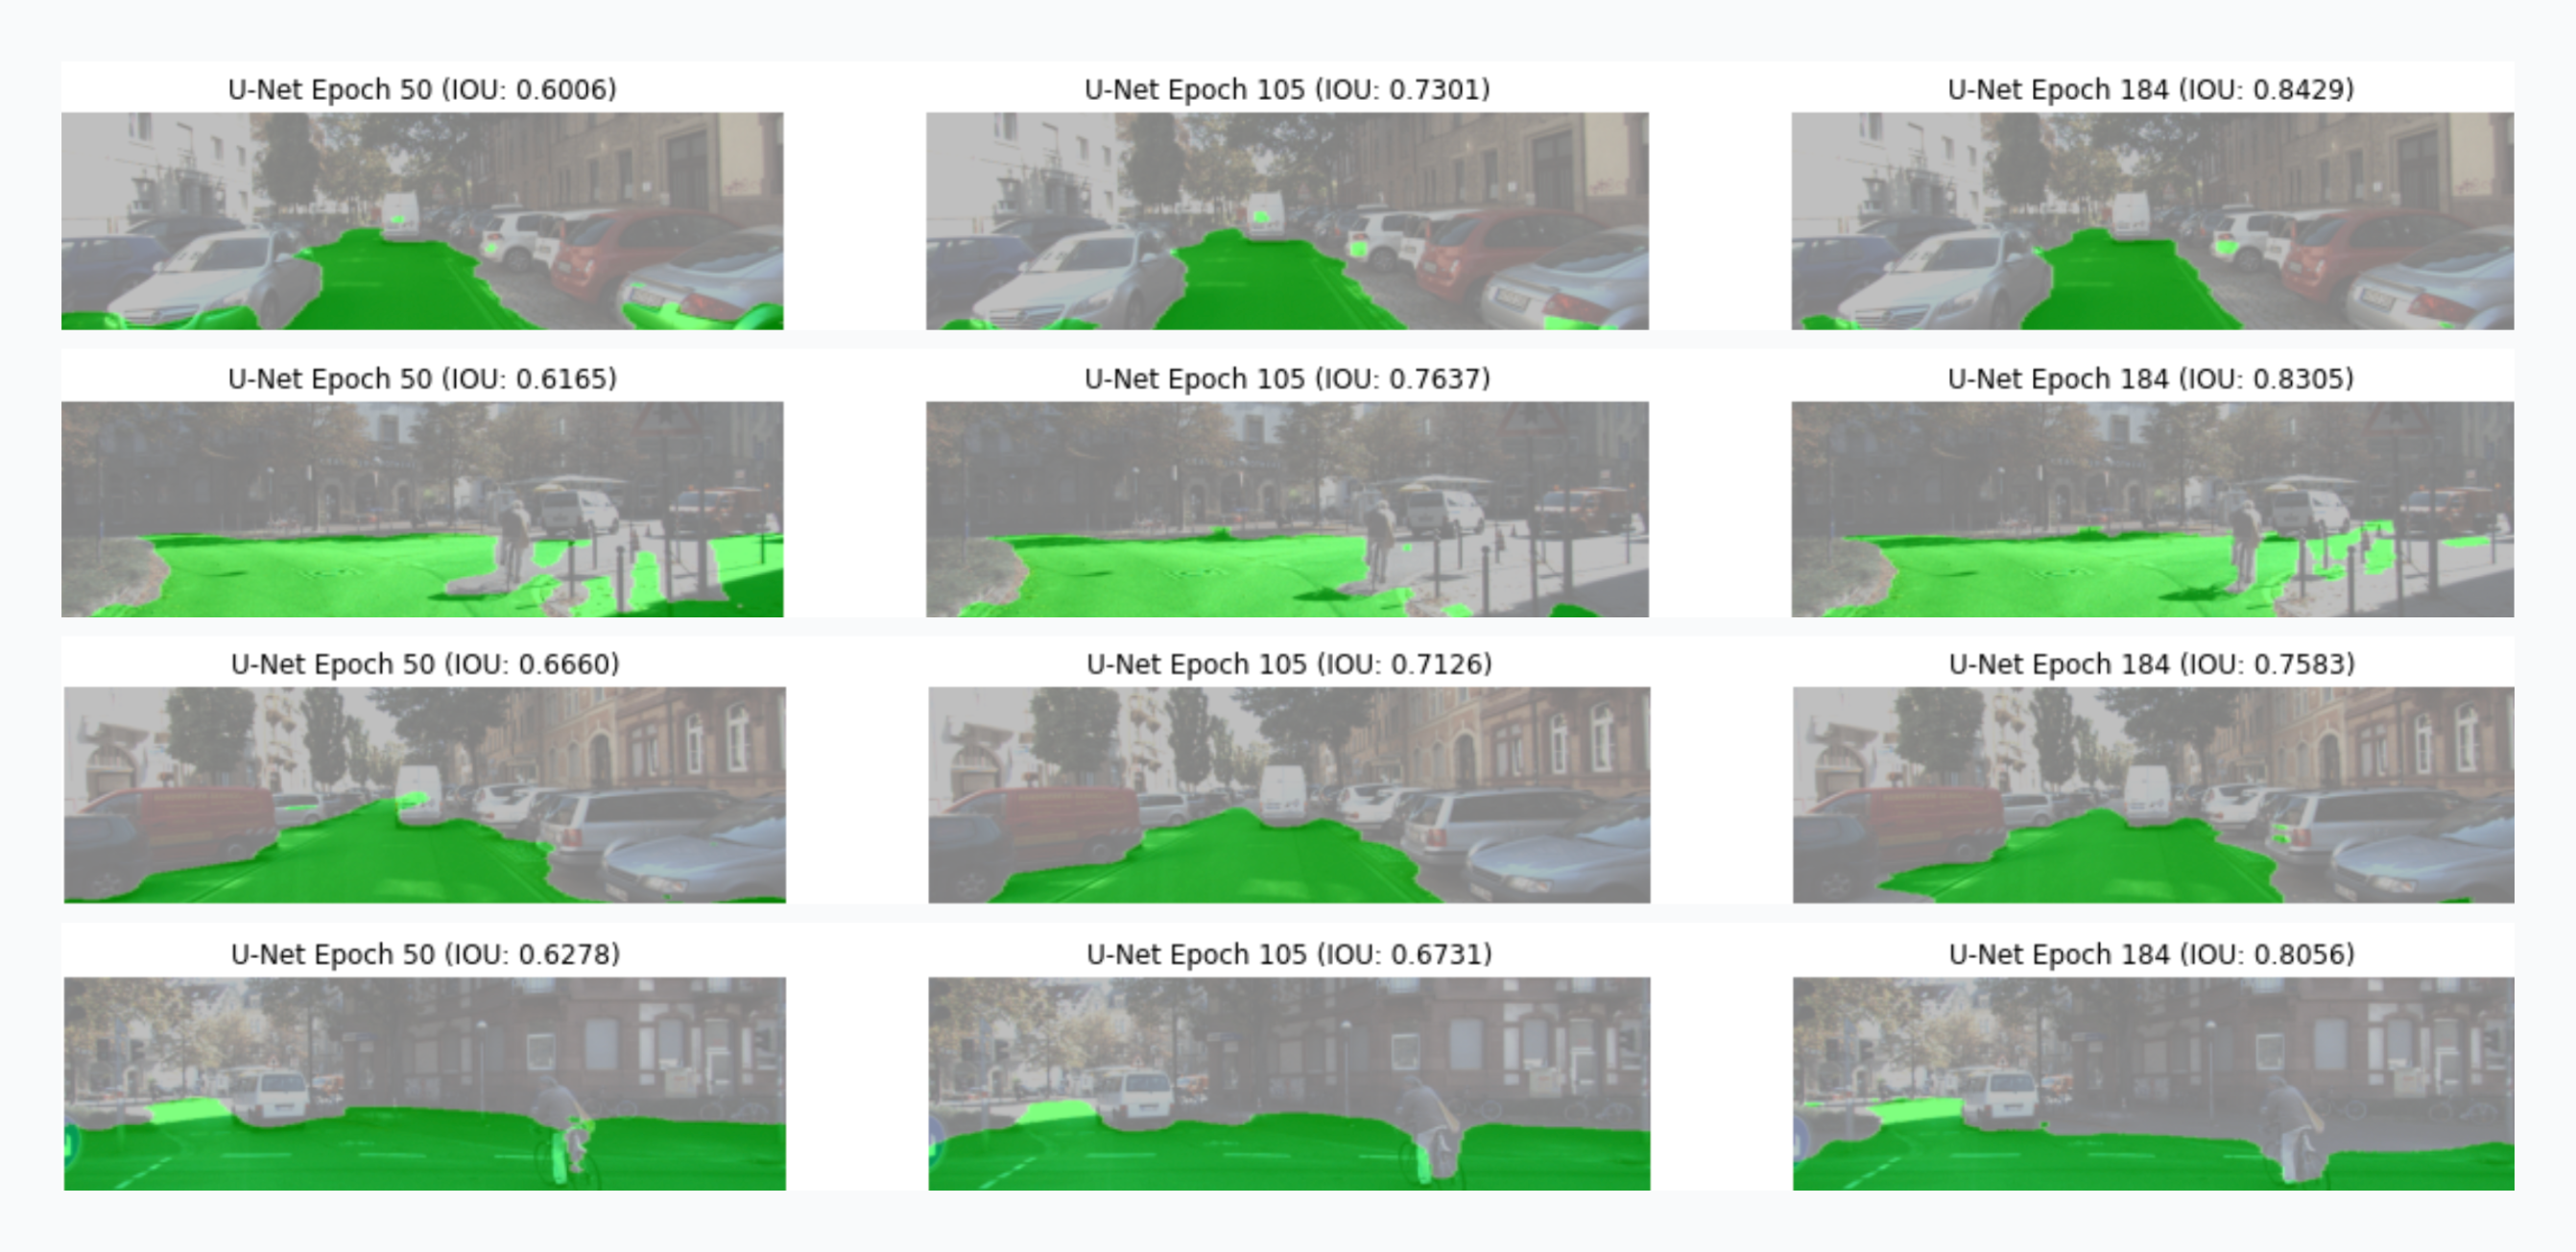
\includegraphics[width=\linewidth]{unet.png}
    \caption{U-Net segmentation results at different epochs. Segmentation results for U-Net by epoch. The results show that the U-Net learns stably until the end epoch. A quantitative evaluation of the change in IOU values is also shown.
 We can see that the highest IOU values are seen at the end.}
    \label{fig:unet_results}
\end{figure}

% 두 번째 그림
\begin{figure}[H]
    \centering
    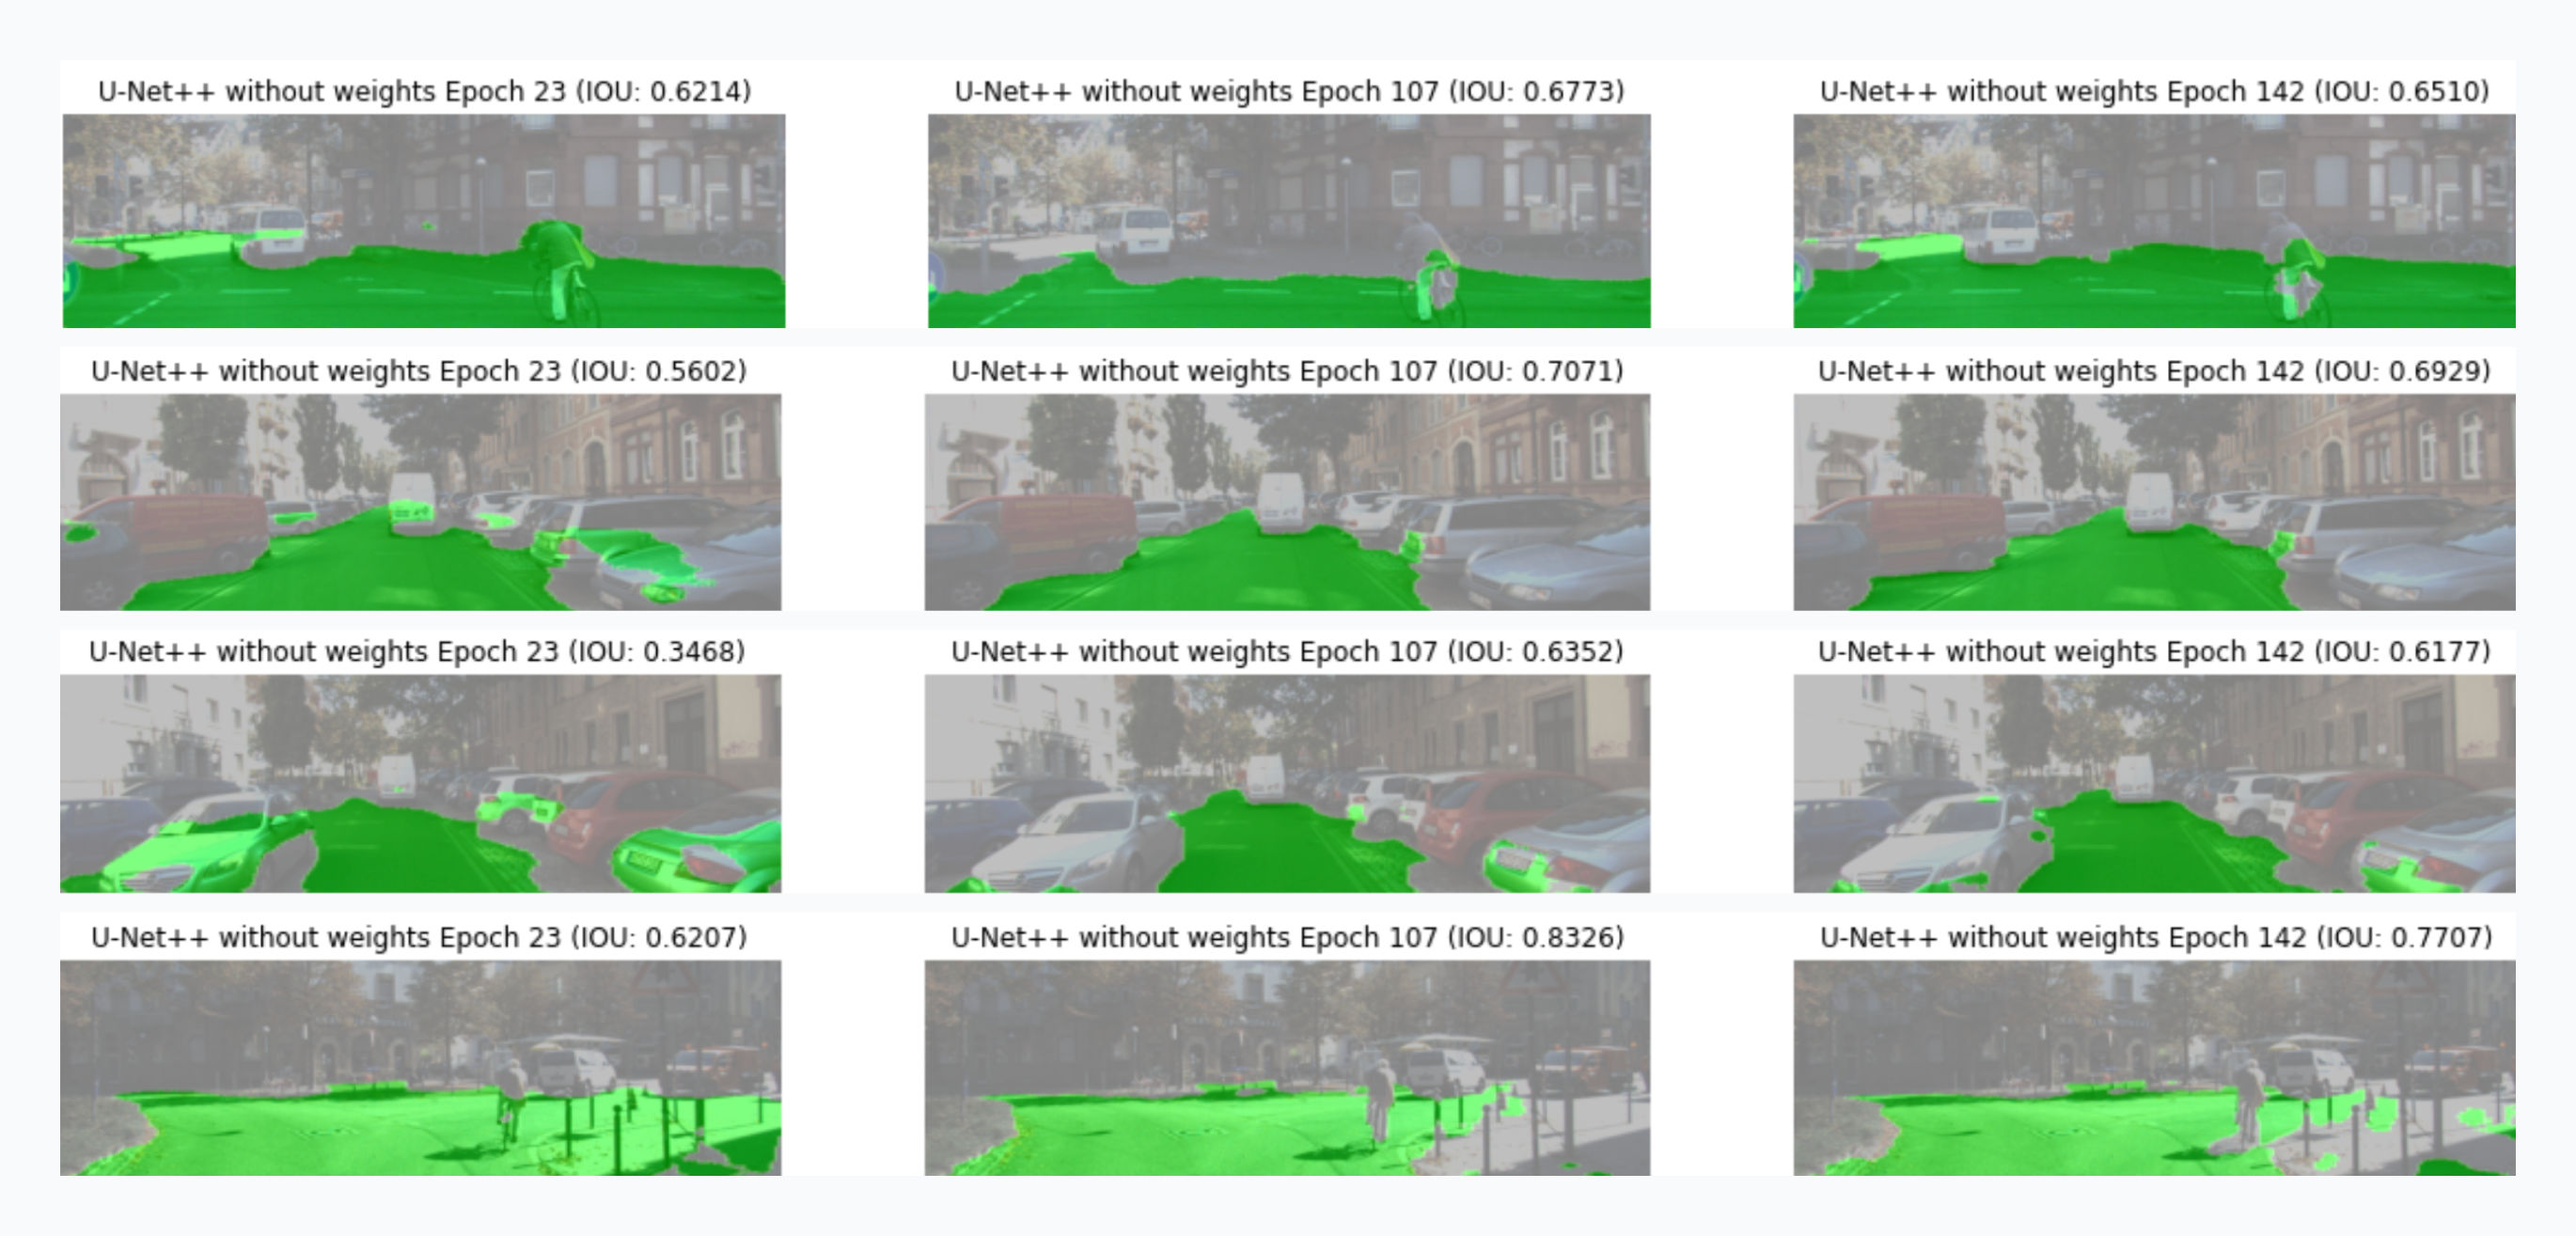
\includegraphics[width=\linewidth]{unet++no.png}
    \caption{U-Net++ segmentation results without pre-trained weights. Unlike U-Net, we see the best quantitative and qualitative performance metrics at the midpoint of training. We can see that the checkpoint model should use a model near the midpoint above.}
    \label{fig:unet++_no_weights}
\end{figure}

% 세 번째 그림
\begin{figure}[H]
    \centering
    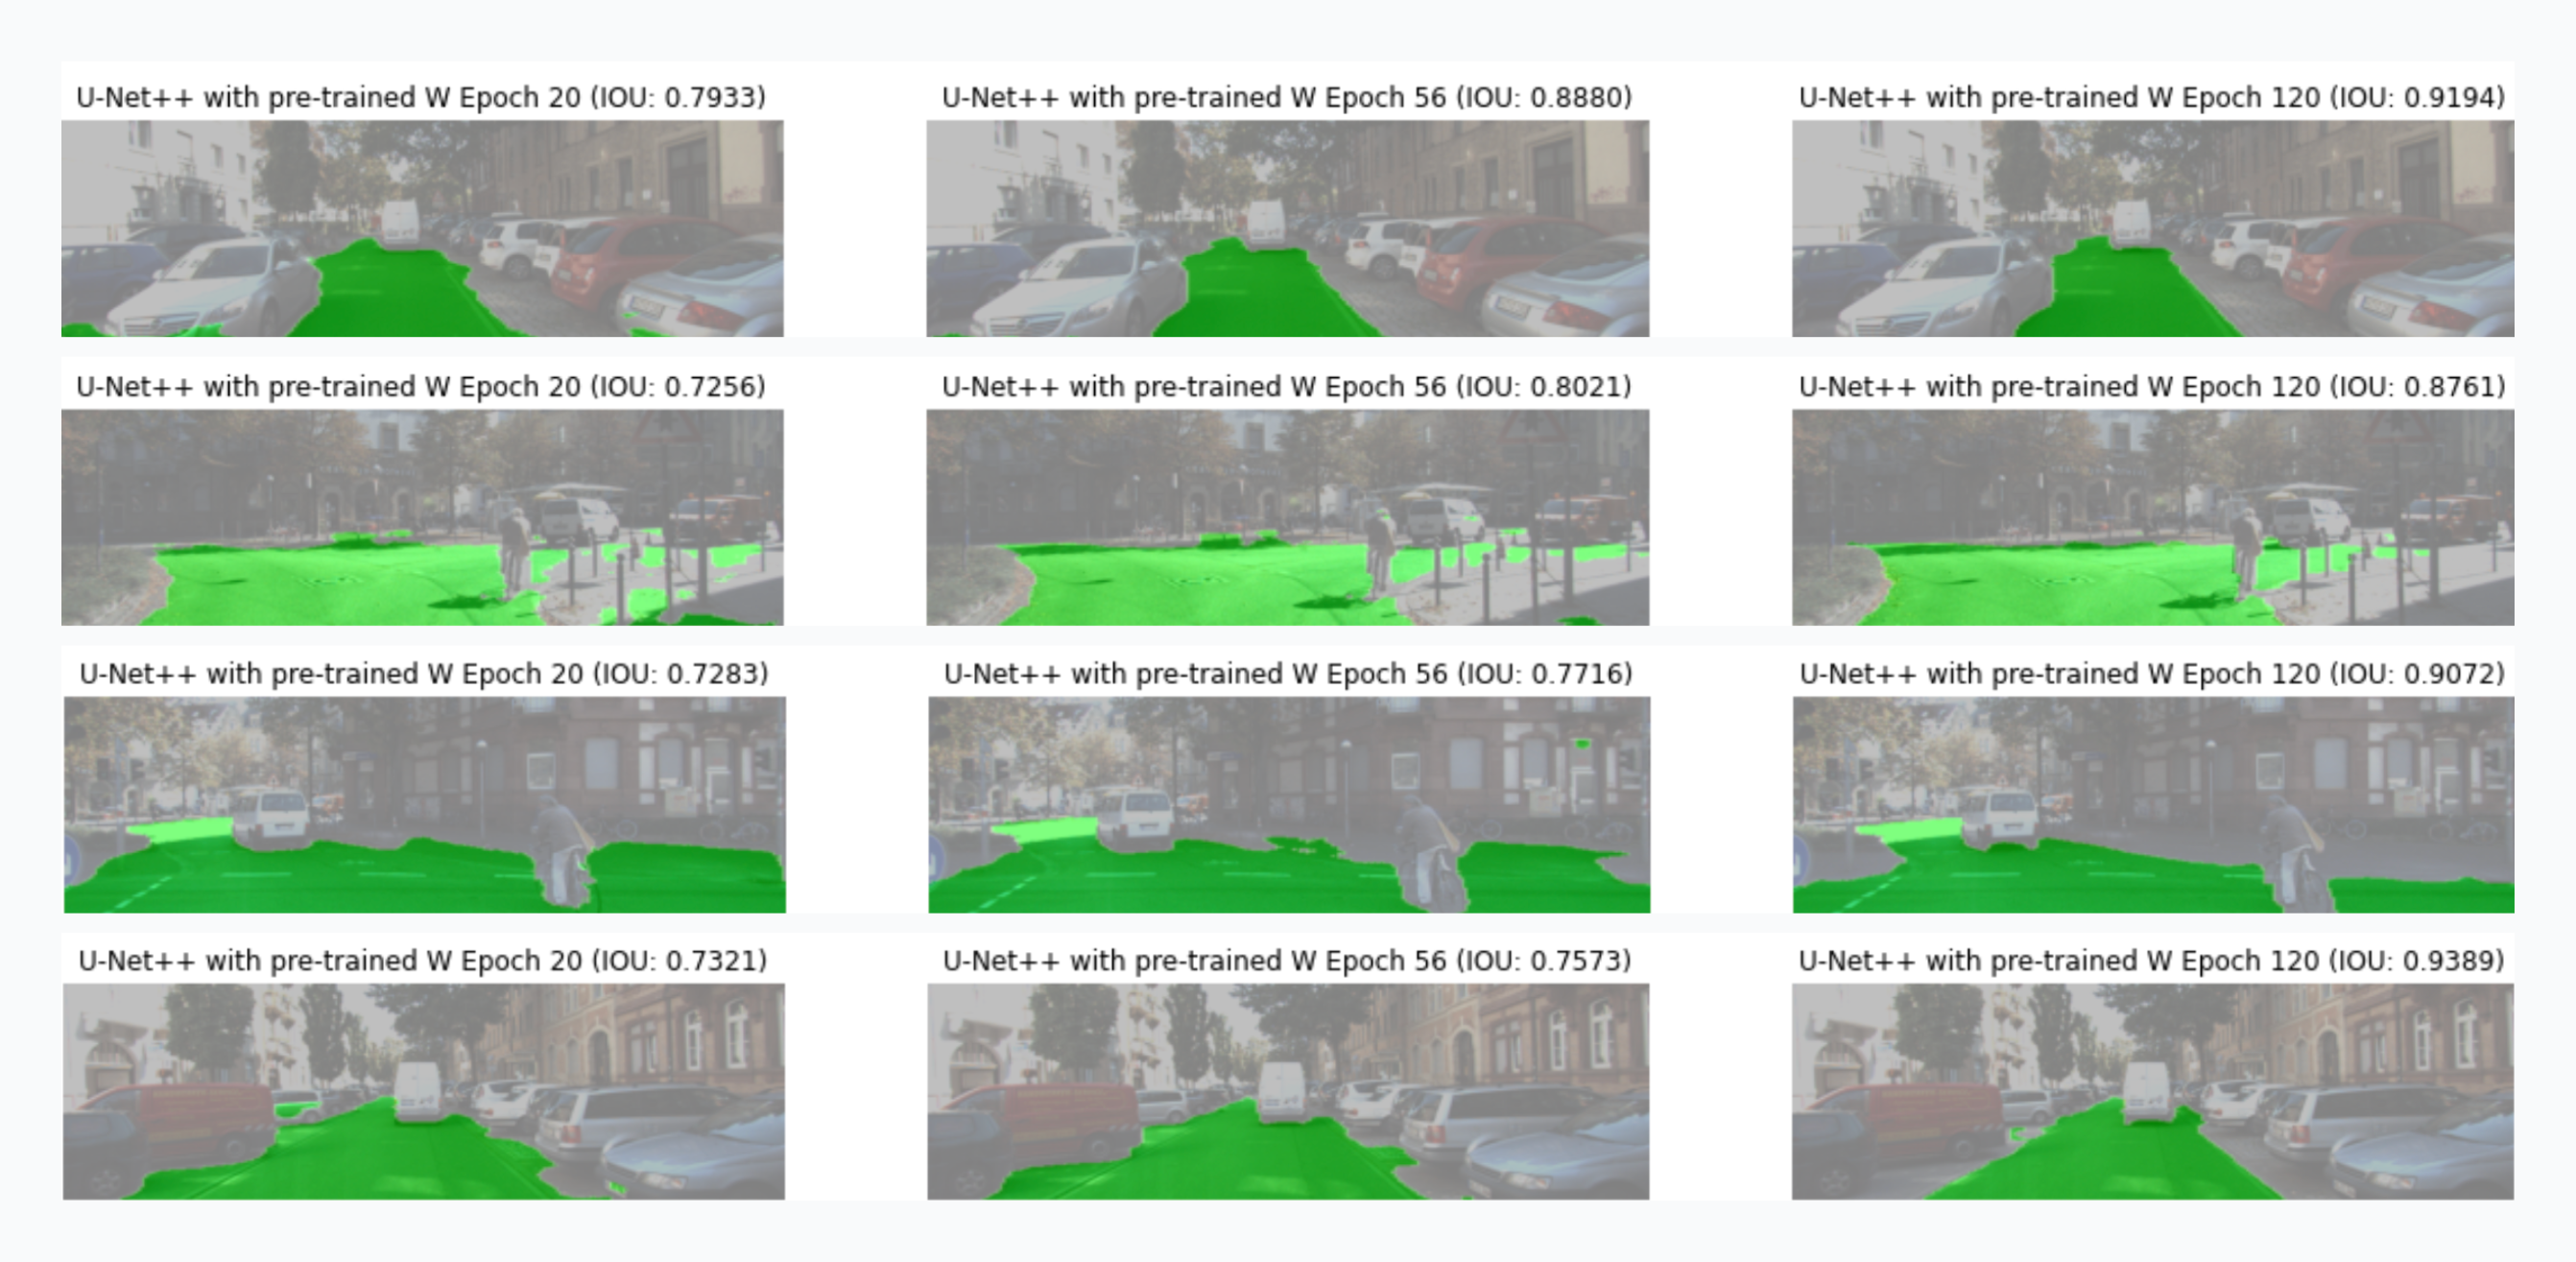
\includegraphics[width=\linewidth]{unet++yes.png}
    \caption{U-Net++ segmentation results with ImageNet pre-trained weights. This configuration demonstrates superior performance, with higher IoU values. }
    \label{fig:unet++_with_weights}
\end{figure}

Figure 1-3 shows the performance of the models for each epoch using quantitative and qualitative metrics. Comparing the performance of each epoch during training provides a basis for selecting the point at which the model is optimized. The average Intersection-over-Union (IoU) value was highest for the UNet++ (using pre-trained weights) model.
 See Table 1 below. This means that the model did a better job of learning the ground truth regions. As a result, it segmented the road regions well.

\vspace{10pt} % 줄과 테이블 사이에 10pt의 간격 추가

\begin{table}[h]
\centering
\caption{Average IoU values for different models.}
\label{tab:iou_comparison}
\begin{tabular}{|c|c|}
\hline
\textbf{Model} & \textbf{Average IoU} \\ \hline
U-Net & 0.8127 \\ \hline
U-Net++ (No Pre-trained Weights) & 0.6807 \\ \hline
U-Net++ (Pre-trained Weights) & 0.9092 \\ \hline
\end{tabular}
\end{table}

\vspace{10pt} % 줄과 테이블 사이에 10pt의 간격 추가

% 네 번째 그림
\begin{figure}[H]
    \centering
    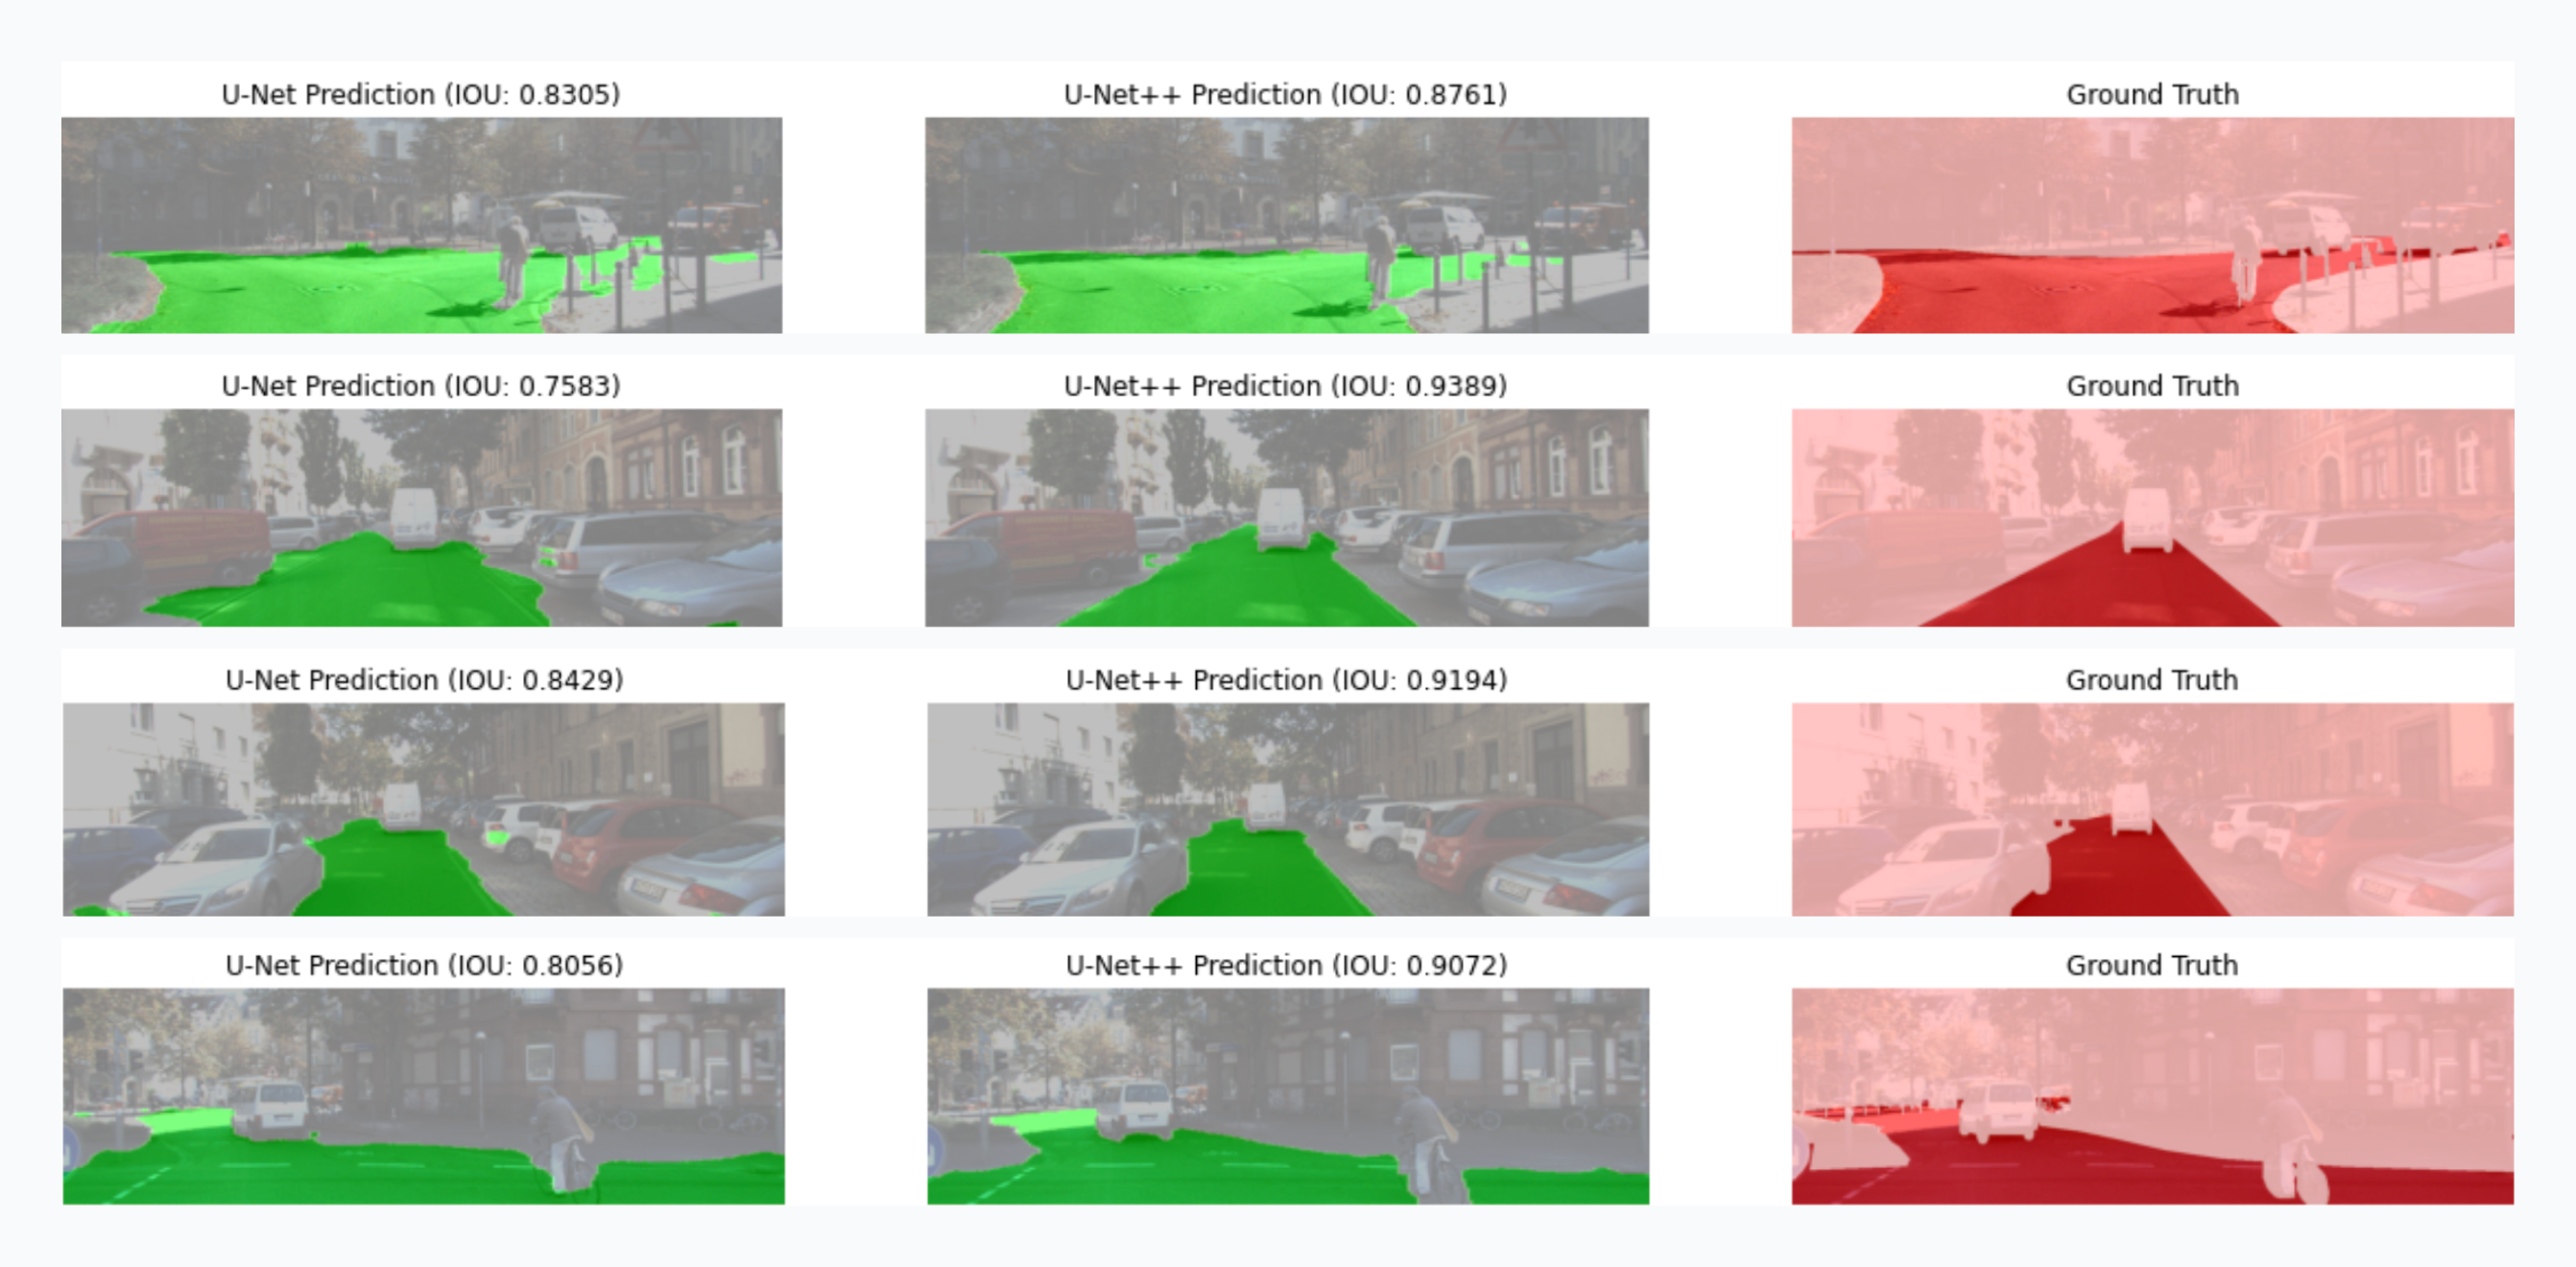
\includegraphics[width=\linewidth]{ground.png}
    \caption{Comparison of predicted segmentation masks and ground truth(Red mask) for U-Net and U-Net++ with ImageNet pre-trained weights. A qualitative comparison shows that the U-Net++ model based on pre-trained weights performs better.  }
    \label{fig:unet++_with_weights}
\end{figure}

Figure 4 above shows a qualitative comparison of the segmentation masks of the top two performing models with the Ground Truth Mask.  We can see that the UNet++ using pre-trained weights model is better at identifying the boundaries of detailed objects such as road boundaries, vehicles, and pedestrians than the original U-Net model.

%-------------------------------------------------------------------------
%%%%%%%%% BODY TEXT
\section{Conclusion}
\label{sec:intro}

These results suggest that the pre-trained weights from the ImageNet dataset were successfully transferred to a new domain such as the KITTI dataset.
The ImageNet dataset consists of various classes such as animals (dogs, cats, elephants), plants (trees, flowers), objects (chairs, cars), and places (beaches, mountains). While these datasets do not directly reflect roadway segmentation, their inclusion of “transportation-related data” can provide indirect learning. In particular, they were an important contribution to learning patterns or features of background objects that should be excluded. This likely helped the model more clearly identify the edges of roads and objects during the segmentation process.
The fact that the UNet++ model with pre-trained weights performed the best shows that this generalized feature learning was successfully transferred to the new domain.  This once again emphasizes that the ImageNet dataset contains a wide range of visual features, and therefore has great potential to be utilized in other datasets or domains.

Additionally, the U-Net++ model (which does not use pre-trained weights) did not clearly outperform the regular U-Net model. 
This suggests that U-Net++, with its nested architecture, may need to be trained on more datasets to outperform the regular U-Net model.

This study centered on the KITTI dataset, U-Net, U-Net++, and VGG16 as the backbone model. However, there are still some limitations, so the following are the directions for future research based on this study.
\textbf{Diversification of backbone models.
}The current study centered on the VGG16 backbone. But replacing the backbone model with 'deeper and newer models' such as ResNet and EfficientNet may further improve performance. In particular, models such as ResNet can efficiently learn from deep networks through residual connections, so we will compare their performance in future studies.

%-------------------------------------------------------------------------
%%%%%%%%% BODY TEXT
\section{Acknowlegements}
\label{sec:intro}
All of the above research was done with the help of our modulab' facilitators and peers.


%-------------------------------------------------------------------------
%%%%%%%%% BODY TEXT
\section{References}
\label{sec:intro}

[1] Olaf Ronneberger, Philipp Fischer, and Thomas Brox. U-Net: Convolutional Networks for Biomedical Image Segmentation. *Medical Image Computing and Computer-Assisted Intervention (MICCAI)*, 2015, pages 234–241.

[2] Zongwei Zhou, Md Mahfuzur Rahman Siddiquee, Nima Tajbakhsh, and Jianming Liang. UNet++: A Nested U-Net Architecture for Medical Image Segmentation. *Deep Learning in Medical Image Analysis and Multimodal Learning for Clinical Decision Support*, 2018, pages 3–11.

[3] Karen Simonyan and Andrew Zisserman. Very Deep Convolutional Networks for Large-Scale Image Recognition. In *International Conference on Learning Representations (ICLR)*, 2015.

[4] Andreas Geiger, Philip Lenz, and Raquel Urtasun. The KITTI Vision Benchmark Suite. *IEEE Conference on Computer Vision and Pattern Recognition (CVPR)*, 2012, pages 3354–3361.

[5] Jia Deng, Wei Dong, Richard Socher, Li-Jia Li, Kai Li, and Li Fei-Fei. ImageNet: A Large-Scale Hierarchical Image Database. *IEEE Conference on Computer Vision and Pattern Recognition (CVPR)*, 2009, pages 248–255.

[6] Zongwei Zhou, Md Mahfuzur Rahman Siddiquee, Nima Tajbakhsh, and Jianming Liang. UNet++: A Nested U-Net Architecture for Medical Image Segmentation. arXiv preprint arXiv:1807.10165, 2018. URL https://arxiv.org/abs/1807.10165.

[7] GitHub Repository for UNet++. URL https://github.com/MrGiovanni/UNetPlusPlus.

\end{document}
%-------------------------------------------------------------------------


\subsection{Mathematics}

Please number all of your sections and displayed equations as in these examples:
\begin{equation}
  E = m\cdot c^2
  \label{eq:important}
\end{equation}
and
\begin{equation}
  v = a\cdot t.
  \label{eq:also-important}
\end{equation}
It is important for readers to be able to refer to any particular equation.
Just because you did not refer to it in the text does not mean some future reader might not need to refer to it.
It is cumbersome to have to use circumlocutions like ``the equation second from the top of page 3 column 1''.
(Note that the ruler will not be present in the final copy, so is not an alternative to equation numbers).
All authors will benefit from reading Mermin's description of how to write mathematics:
\url{http://www.pamitc.org/documents/mermin.pdf}.

\subsection{Blind review}

Many authors misunderstand the concept of anonymizing for blind review.
Blind review does not mean that one must remove citations to one's own work---in fact it is often impossible to review a paper unless the previous citations are known and available.

Blind review means that you do not use the words ``my'' or ``our'' when citing previous work.
That is all.
(But see below for tech reports.)

Saying ``this builds on the work of Lucy Smith [1]'' does not say that you are Lucy Smith;
it says that you are building on her work.
If you are Smith and Jones, do not say ``as we show in [7]'', say ``as Smith and Jones show in [7]'' and at the end of the paper, include reference 7 as you would any other cited work.

An example of a bad paper just asking to be rejected:
\begin{quote}
\begin{center}
    An analysis of the frobnicatable foo filter.
\end{center}

   In this paper we present a performance analysis of our previous paper [1], and show it to be inferior to all previously known methods.
   Why the previous paper was accepted without this analysis is beyond me.

   [1] Removed for blind review
\end{quote}


An example of an acceptable paper:
\begin{quote}
\begin{center}
     An analysis of the frobnicatable foo filter.
\end{center}

   In this paper we present a performance analysis of the  paper of Smith \etal [1], and show it to be inferior to all previously known methods.
   Why the previous paper was accepted without this analysis is beyond me.

   [1] Smith, L and Jones, C. ``The frobnicatable foo filter, a fundamental contribution to human knowledge''. Nature 381(12), 1-213.
\end{quote}

If you are making a submission to another conference at the same time, which covers similar or overlapping material, you may need to refer to that submission in order to explain the differences, just as you would if you had previously published related work.
In such cases, include the anonymized parallel submission~\cite{Authors14} as supplemental material and cite it as
\begin{quote}
[1] Authors. ``The frobnicatable foo filter'', F\&G 2014 Submission ID 324, Supplied as supplemental material {\tt fg324.pdf}.
\end{quote}

Finally, you may feel you need to tell the reader that more details can be found elsewhere, and refer them to a technical report.
For conference submissions, the paper must stand on its own, and not {\em require} the reviewer to go to a tech report for further details.
Thus, you may say in the body of the paper ``further details may be found in~\cite{Authors14b}''.
Then submit the tech report as supplemental material.
Again, you may not assume the reviewers will read this material.

Sometimes your paper is about a problem which you tested using a tool that is widely known to be restricted to a single institution.
For example, let's say it's 1969, you have solved a key problem on the Apollo lander, and you believe that the CVPR70 audience would like to hear about your
solution.
The work is a development of your celebrated 1968 paper entitled ``Zero-g frobnication: How being the only people in the world with access to the Apollo lander source code makes us a wow at parties'', by Zeus \etal.

You can handle this paper like any other.
Do not write ``We show how to improve our previous work [Anonymous, 1968].
This time we tested the algorithm on a lunar lander [name of lander removed for blind review]''.
That would be silly, and would immediately identify the authors.
Instead write the following:
\begin{quotation}
\noindent
   We describe a system for zero-g frobnication.
   This system is new because it handles the following cases:
   A, B.  Previous systems [Zeus et al. 1968] did not  handle case B properly.
   Ours handles it by including a foo term in the bar integral.

   ...

   The proposed system was integrated with the Apollo lunar lander, and went all the way to the moon, don't you know.
   It displayed the following behaviours, which show how well we solved cases A and B: ...
\end{quotation}
As you can see, the above text follows standard scientific convention, reads better than the first version, and does not explicitly name you as the authors.
A reviewer might think it likely that the new paper was written by Zeus \etal, but cannot make any decision based on that guess.
He or she would have to be sure that no other authors could have been contracted to solve problem B.
\medskip

\noindent
FAQ\medskip\\
{\bf Q:} Are acknowledgements OK?\\
{\bf A:} No.  Leave them for the final copy.\medskip\\
{\bf Q:} How do I cite my results reported in open challenges?
{\bf A:} To conform with the double-blind review policy, you can report results of other challenge participants together with your results in your paper.
For your results, however, you should not identify yourself and should not mention your participation in the challenge.
Instead present your results referring to the method proposed in your paper and draw conclusions based on the experimental comparison to other results.\medskip\\

\begin{figure}[t]
  \centering
  \fbox{\rule{0pt}{2in} \rule{0.9\linewidth}{0pt}}
   %\includegraphics[width=0.8\linewidth]{egfigure.eps}

   \caption{Example of caption.
   It is set in Roman so that mathematics (always set in Roman: $B \sin A = A \sin B$) may be included without an ugly clash.}
   \label{fig:onecol}
\end{figure}

\subsection{Miscellaneous}

\noindent
Compare the following:\\
\begin{tabular}{ll}
 \verb'$conf_a$' &  $conf_a$ \\
 \verb'$\mathit{conf}_a$' & $\mathit{conf}_a$
\end{tabular}\\
See The \TeX book, p165.

The space after \eg, meaning ``for example'', should not be a sentence-ending space.
So \eg is correct, {\em e.g.} is not.
The provided \verb'\eg' macro takes care of this.

When citing a multi-author paper, you may save space by using ``et alia'', shortened to ``\etal'' (not ``{\em et.\ al.}'' as ``{\em et}'' is a complete word).
If you use the \verb'\etal' macro provided, then you need not worry about double periods when used at the end of a sentence as in Alpher \etal.
However, use it only when there are three or more authors.
Thus, the following is correct:
   ``Frobnication has been trendy lately.
   It was introduced by Alpher~\cite{Alpher02}, and subsequently developed by
   Alpher and Fotheringham-Smythe~\cite{Alpher03}, and Alpher \etal~\cite{Alpher04}.''

This is incorrect: ``... subsequently developed by Alpher \etal~\cite{Alpher03} ...'' because reference~\cite{Alpher03} has just two authors.


% Update the cvpr.cls to do the following automatically.
% For this citation style, keep multiple citations in numerical (not
% chronological) order, so prefer \cite{Alpher03,Alpher02,Authors14} to
% \cite{Alpher02,Alpher03,Authors14}.


\begin{figure*}
  \centering
  \begin{subfigure}{0.68\linewidth}
    \fbox{\rule{0pt}{2in} \rule{.9\linewidth}{0pt}}
    \caption{An example of a subfigure.}
    \label{fig:short-a}
  \end{subfigure}
  \hfill
  \begin{subfigure}{0.28\linewidth}
    \fbox{\rule{0pt}{2in} \rule{.9\linewidth}{0pt}}
    \caption{Another example of a subfigure.}
    \label{fig:short-b}
  \end{subfigure}
  \caption{Example of a short caption, which should be centered.}
  \label{fig:short}
\end{figure*}

%------------------------------------------------------------------------
\section{Formatting your paper}
\label{sec:formatting}

All text must be in a two-column format.
The total allowable size of the text area is $6\frac78$ inches (17.46 cm) wide by $8\frac78$ inches (22.54 cm) high.
Columns are to be $3\frac14$ inches (8.25 cm) wide, with a $\frac{5}{16}$ inch (0.8 cm) space between them.
The main title (on the first page) should begin 1 inch (2.54 cm) from the top edge of the page.
The second and following pages should begin 1 inch (2.54 cm) from the top edge.
On all pages, the bottom margin should be $1\frac{1}{8}$ inches (2.86 cm) from the bottom edge of the page for $8.5 \times 11$-inch paper;
for A4 paper, approximately $1\frac{5}{8}$ inches (4.13 cm) from the bottom edge of the
page.

%-------------------------------------------------------------------------
\subsection{Margins and page numbering}

All printed material, including text, illustrations, and charts, must be kept
within a print area $6\frac{7}{8}$ inches (17.46 cm) wide by $8\frac{7}{8}$ inches (22.54 cm)
high.
%
Page numbers should be in the footer, centered and $\frac{3}{4}$ inches from the bottom of the page.
The review version should have page numbers, yet the final version submitted as camera ready should not show any page numbers.
The \LaTeX\ template takes care of this when used properly.



%-------------------------------------------------------------------------
\subsection{Type style and fonts}

Wherever Times is specified, Times Roman may also be used.
If neither is available on your word processor, please use the font closest in
appearance to Times to which you have access.

MAIN TITLE.
Center the title $1\frac{3}{8}$ inches (3.49 cm) from the top edge of the first page.
The title should be in Times 14-point, boldface type.
Capitalize the first letter of nouns, pronouns, verbs, adjectives, and adverbs;
do not capitalize articles, coordinate conjunctions, or prepositions (unless the title begins with such a word).
Leave two blank lines after the title.

AUTHOR NAME(s) and AFFILIATION(s) are to be centered beneath the title
and printed in Times 12-point, non-boldface type.
This information is to be followed by two blank lines.

The ABSTRACT and MAIN TEXT are to be in a two-column format.

MAIN TEXT.
Type main text in 10-point Times, single-spaced.
Do NOT use double-spacing.
All paragraphs should be indented 1 pica (approx.~$\frac{1}{6}$ inch or 0.422 cm).
Make sure your text is fully justified---that is, flush left and flush right.
Please do not place any additional blank lines between paragraphs.

Figure and table captions should be 9-point Roman type as in \cref{fig:onecol,fig:short}.
Short captions should be centred.

\noindent Callouts should be 9-point Helvetica, non-boldface type.
Initially capitalize only the first word of section titles and first-, second-, and third-order headings.

FIRST-ORDER HEADINGS.
(For example, {\large \bf 1. Introduction}) should be Times 12-point boldface, initially capitalized, flush left, with one blank line before, and one blank line after.

SECOND-ORDER HEADINGS.
(For example, { \bf 1.1. Database elements}) should be Times 11-point boldface, initially capitalized, flush left, with one blank line before, and one after.
If you require a third-order heading (we discourage it), use 10-point Times, boldface, initially capitalized, flush left, preceded by one blank line, followed by a period and your text on the same line.

%-------------------------------------------------------------------------
\subsection{Footnotes}

Please use footnotes\footnote{This is what a footnote looks like.
It often distracts the reader from the main flow of the argument.} sparingly.
Indeed, try to avoid footnotes altogether and include necessary peripheral observations in the text (within parentheses, if you prefer, as in this sentence).
If you wish to use a footnote, place it at the bottom of the column on the page on which it is referenced.
Use Times 8-point type, single-spaced.


%-------------------------------------------------------------------------
\subsection{Cross-references}

For the benefit of author(s) and readers, please use the
{\small\begin{verbatim}
  \cref{...}
\end{verbatim}}  command for cross-referencing to figures, tables, equations, or sections.
This will automatically insert the appropriate label alongside the cross-reference as in this example:
\begin{quotation}
  To see how our method outperforms previous work, please see \cref{fig:onecol} and \cref{tab:example}.
  It is also possible to refer to multiple targets as once, \eg~to \cref{fig:onecol,fig:short-a}.
  You may also return to \cref{sec:formatting} or look at \cref{eq:also-important}.
\end{quotation}
If you do not wish to abbreviate the label, for example at the beginning of the sentence, you can use the
{\small\begin{verbatim}
  \Cref{...}
\end{verbatim}}
command. Here is an example:
\begin{quotation}
  \Cref{fig:onecol} is also quite important.
\end{quotation}

%-------------------------------------------------------------------------
\subsection{References}

List and number all bibliographical references in 9-point Times, single-spaced, at the end of your paper.
When referenced in the text, enclose the citation number in square brackets, for
example~\cite{Authors14}.
Where appropriate, include page numbers and the name(s) of editors of referenced books.
When you cite multiple papers at once, please make sure that you cite them in numerical order like this \cite{Alpher02,Alpher03,Alpher05,Authors14b,Authors14}.
If you use the template as advised, this will be taken care of automatically.

\begin{table}
  \centering
  \begin{tabular}{@{}lc@{}}
    \toprule
    Method & Frobnability \\
    \midrule
    Theirs & Frumpy \\
    Yours & Frobbly \\
    Ours & Makes one's heart Frob\\
    \bottomrule
  \end{tabular}
  \caption{Results.   Ours is better.}
  \label{tab:example}
\end{table}

%-------------------------------------------------------------------------
\subsection{Illustrations, graphs, and photographs}

All graphics should be centered.
In \LaTeX, avoid using the \texttt{center} environment for this purpose, as this adds potentially unwanted whitespace.
Instead use
{\small\begin{verbatim}
  \centering
\end{verbatim}}
at the beginning of your figure.
Please ensure that any point you wish to make is resolvable in a printed copy of the paper.
Resize fonts in figures to match the font in the body text, and choose line widths that render effectively in print.
Readers (and reviewers), even of an electronic copy, may choose to print your paper in order to read it.
You cannot insist that they do otherwise, and therefore must not assume that they can zoom in to see tiny details on a graphic.

When placing figures in \LaTeX, it's almost always best to use \verb+\includegraphics+, and to specify the figure width as a multiple of the line width as in the example below
{\small\begin{verbatim}
   \usepackage{graphicx} ...
   \includegraphics[width=0.8\linewidth]
                   {myfile.pdf}
\end{verbatim}
}


%-------------------------------------------------------------------------
\subsection{Color}

Please refer to the author guidelines on the \confName\ \confYear\ web page for a discussion of the use of color in your document.

If you use color in your plots, please keep in mind that a significant subset of reviewers and readers may have a color vision deficiency; red-green blindness is the most frequent kind.
Hence avoid relying only on color as the discriminative feature in plots (such as red \vs green lines), but add a second discriminative feature to ease disambiguation.

%------------------------------------------------------------------------
\section{Final copy}

You must include your signed IEEE copyright release form when you submit your finished paper.
We MUST have this form before your paper can be published in the proceedings.

Please direct any questions to the production editor in charge of these proceedings at the IEEE Computer Society Press:
\url{https://www.computer.org/about/contact}.


%%%%%%%%% REFERENCES
{\small
\bibliographystyle{ieee_fullname}
\bibliography{egbib}
}

\end{document}
